\documentclass{article}

\usepackage{amsmath}
\usepackage{amssymb}
\usepackage{parskip}
\usepackage{fullpage}
\usepackage{hyperref}
\usepackage{tikz}
\usepackage{wrapfig}
\usepackage{bettelini}

\usetikzlibrary{ % tikz packages
    automata,positioning,
    arrows.meta,bending
}

\hypersetup{
    colorlinks=true,
    linkcolor=black,
    urlcolor=blue,
    pdftitle={TheoryOfComputation},
    pdfpagemode=FullScreen,
}

\tikzset{every state/.style={
    inner sep=2pt,
    minimum size=4pt
}}
\tikzset{>=stealth}  %latex, to, stealth

\title{Theory of Computation}
\author{Paolo Bettelini}
\date{}

% Empty string symbol.
\newcommand{\emptyString}{\lambda}

\begin{document}

\maketitle
\tableofcontents
\pagebreak

\section{Fields of Study}

\subsection{Complexity Theory}

Classify problems according to their degree
of "difficulty".

\subsection{Computability Theory}

Classify problems as being solvable or unsolvable.

\subsection{Automata Theory}

Compare different computation models.

\section{Alphabets and Languages}

An \textit{alphabet} is a finite set of \textit{symbols}.
For example: \(\{a,b,c,\cdots, z\}\)\\
The set \(\{0,1\}\) is the binary set.
The empty string is denoted \(\emptyString\).
\\
Note that \(\emptyString \neq \varnothing \neq \{\emptyString\}\).
\\
The length of a string \(w\) is denoted as \(|w|\).

If \(\Sigma\) is an alphabet,
\[
    \Sigma_\emptyString = \emptyString \union \Sigma
\]

A set of strings is called a \textit{language}.

\section{Deterministic Finite Automaton}

A deterministic finite automaton (DFA) is a state-machine which processes a string
symbol by symbol from left to right. The automaton is in one of his \textit{states}
after processing a symbol. The machine might terminate in an
\textit{accept state} or not.

A DFA \(M=(Q, \Sigma, \delta, q, F)\)
\begin{itemize}
    \item \(Q\) is a finite set of \textit{states}
    \item \(\Sigma\) is an alphabet
    \item \(\delta : Q \times \Sigma \to Q\) is the \textit{transition function}
    \item \(q\) is an element of \(Q\) called the \textit{start state}
    \item \(F\) is a subset of \(Q\) which contains the \textit{accept states}
\end{itemize}
The transition function is the logical components, it determines
in which state the machine will be after processing a symbol at any state.

The following automaton processes a binary string.
The start state is \(q_1\) and the only accept state is \(q_3\).
The program moves to the next state only if the symbol is \(1\),
so it will reach \(q_3\) only if the input string contains at least two \(1\)s.
\begin{center}
    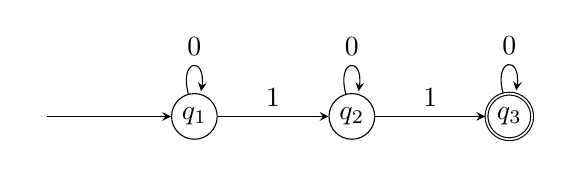
\begin{tikzpicture}[node distance=2cm,on grid,auto]
        \node[state] (q1) {\(q_1\)};
        \node (inv) [left=of q1] {};

        \node[state] (q2) [right=of q1] {\(q_2\)};
        \node[state, accepting] (q3) [right=of q2] {\(q_3\)};

        \path[->]
            (inv)
                edge node {} (q1)
            (q1)
                edge node {\(1\)} (q2)
                edge[loop above] node {\(0\)} ()
            (q2)
                edge node {\(1\)} (q3)
                edge[loop above] node {\(0\)} ()
            (q3)
                edge[loop above] node {\(0\)} ();
    \end{tikzpicture}
\end{center}


If a DFA is in a state \(r\) and it reads the symbol \(a\),
then it will uniquely switch to the state \(\delta(r, a)\)

\pagebreak

The language of \(M\), denoted \(L(M)\) is the set of all accepted strings
by \(M\).
\[
    L(M) = \{w \in \Sigma^* \suchthat M\text{ accepts }w\}
\]

\section{Operations}

\subsection{Concatenation}

If \(A\) and \(B\) are two languages over the same alphabet,
the concatenation of \(A\) and \(B\) is defined as
\[
    AB = \{ab \suchthat a \in A \land b \in B\}
\]

\subsection{Kleene star operator}

The kleene star operator can be applied to alphabets or languages.
It represent the union of all \(n\)-permutations of the set. \\
The set \(\{0,1\}^*\) is the set of
all binary strings. If \(\Sigma\) is an alphabet, \(\Sigma^*\) is the set
of all strings over \(\Sigma\)
\[
    \Sigma^* = \emptyString \cup \bigcup_{n\in\mathbb{N}} \Sigma^n
\]

\section{Regular language}

A language is regular if an automaton that accepts said language exists.
\(A\) is regular iff
\[
    \exists M \suchthat L(M) = A
\]

\subsection{Closure under union (extra)}

\textit{If \(A\) and \(B\) are two regular languages over the same alphabet
\(\Sigma\), then \(A \union B\) is also regular.}

We can prove this by making a DFA that accepts both languages.
Let's say that \(M_1=(Q_1, \Sigma, \delta_1, q_1, F_1)\) accepts \(A\)
and \(M_2=(Q_2, \Sigma, \delta_2, q_2, F_2)\) accepts \(B\).
The automaton \(M=(Q, \Sigma, \delta, q, F)\) must run \(M_1\) and \(M_2\) \textit{simultaneously},
so any state must represent the current states of \(M_1\) and \(M_2\).
This means that the states of \(M\) must represent any combination of state between
\(M_1\) and \(M_2\), meaning \(Q=Q_1 \times Q_2\).
The transition function is now in the form
\(\delta((r_1, r_2), a) = (\delta_1(r_1, a), \delta_2(r_2, a))\) where \(a\in\Sigma\).
The initial state is the state in \(Q\) which contains the initial state of \(M_1\)
and \(M_2\), namely \((q_1, q_2)\). Finally, the set of accept states
is every tuple in \(Q_1\) containing a state in \(F_2\) or in \(Q_2\) containing a state in \(F_1\), namely
\(Q_1 \times F_2 \union Q_2 \times F_1\). \\
We can conclude that \(M=(Q_1 \times Q_2, \Sigma, \delta((r_1, r_2), a), (q_1, q_2), Q_1 \times F_2 \union Q_2 \times F_1)\)
accepts \(A \union B\) so \(A \union B\) is regular.

\pagebreak

\section{Nondeterministic Finite Automaton}

Nondeterministic finite automata (NFA) are state-machines
like DFAs but can change multiple states at a time by processing
empty strings \(\emptyString\) and when processing a symbol
\(a\) may have multiple possible states to switch to.
The NFA will choose the "correct" switch in order to end in an accept state, if possible.

The following automaton where \(\Sigma = \{1\}\) will end in an accept state
if the input has length which is a multiple of \(2\) or \(3\).

\newcommand\double[3][10]{%
  \draw (#2)
    edge [bend left=#1,draw=none]
    coordinate[at start](#2-#3-s)
    coordinate[at end](#2-#3-e)
    (#3)
    edge [bend right=#1,draw=none]
    coordinate[at start](#3-#2-e)
    coordinate[at end](#3-#2-s)
    (#3);
}

\begin{center}
    \begin{tikzpicture}[node distance=2cm,on grid,auto]
        \node[state] (0) {};
        \node (inv) [left=of 0] {};

        \node[state, accepting] (a1) [above right=of 0] {\(q_{a1}\)};
        \node[state] (a2) [right=of a1] {\(q_{a2}\)};
        
        \node[state, accepting] (b1) [below right=of 0] {\(q_{b1}\)};
        \node[state] (b2) [right=of b1] {\(q_{b2}\)};
        \node[state] (b3) [below=of b2] {\(q_{b3}\)};
        
        \double{a1}{a2};

        \path[->]
            (inv)
                edge node {} (0)
            (0)
                edge node {\(\emptyString\)} (a1)
                edge node {\(\emptyString\)} (b1)
            (a1-a2-s)
                edge node {\(1\)} (a1-a2-e)
            (a2-a1-s)
                edge node {\(1\)} (a2-a1-e)
            (b1)
                edge node {\(1\)} (b2)
            (b2)
                edge node {\(1\)} (b3)
            (b3)
                edge node {\(1\)} (b1);
    \end{tikzpicture}
\end{center}
The first switch is done by processing an empty string and the direction is chosen magically
in order to end in an accept state.

A NFA is defined as \(M=(Q, \Sigma, \delta, q, F)\) where
\begin{itemize}
    \item \(Q\) is a finite set of \textit{states}
    \item \(\Sigma\) is an alphabet
    \item \(\delta : Q \times \Sigma_\emptyString \to \mathcal{P}(Q)\) is the \textit{transition function}
    \item \(q\) is an element of \(Q\) called the \textit{start state}
    \item \(F\) is a subset of \(Q\) which contains the \textit{accept states}
\end{itemize}

\section{Equivalente of DFAs and NFAs}

Anything that can be computed by a NFA can also be computed by a DFA and vice versa.

\subsection{DFA to NFA conversion}

Let \(M=(Q, \Sigma, \delta, q, F)\) be a DFA.
\(\delta\) is not a transition function of a NFA, so we need to redefine it as \(\delta'\).
Since \(\delta\) cannot process \(\emptyString\), \(\delta'\)
it is defined as
\[
    \delta'(r, a)=
    \begin{cases} 
        \delta(r, a) & x \neq \emptyString \\
        \emptyset & x = \emptyString
    \end{cases}
\]
where \(r\) is a state in \(Q\) and \(a\) is a symbol in \(\Sigma_\emptyString\). \\
We can conclude that \(N=(Q, \Sigma, \delta', q, F)\).

\subsection{NFA to DFA conversion}

Let \(N=(Q, \Sigma, \delta, q, F)\) be a NFA. The idea is to construct a DFA \(M=(Q', \Sigma, \delta', q', F')\)
that runs all the possible combinations that could be run by \(N\) at the same time.
Any state of \(M\) is a set of states \(R \in \mathcal{P}(Q)\), so we will say that
\(Q'=\mathcal{P}(Q)\). The set of accept states is any state \(R\) which contains an accept
state of \(N\)
\[
    F' = \{R \in Q' \suchthat R \intersection F \neq \emptyset\}
\]
Let's assume that \(N\) does not execute any \(\emptyString\)-transitions.
\(q'\) would be \(\{q\}\) and \(\delta'\) would be
\[
    \delta'(R, a) = \bigcup_{r\in R}\delta(r,a)
\]
which is the union of all possible states \(N\) could switch to.
Recall that for every \(r\in R\), \(\delta(r,a)\) is a set
of all possible states to switch to.

Let's now remove the previous assumption. Now, \(M\)
must also consider every state that could be reached by
making zero or more \(\emptyString\)-transitions.
The \(\emptyString\)-closure
for a state \(r\), \(C_\emptyString(r)\), is defined as
the set of all possible states that can be reached from \(r\) by making
zero or more \(\emptyString\)-transitions.
The \(\emptyString\)-closure for a set of states \(R\) is defined as
\[
    C_\emptyString(R) = \bigcup_{r\in R}C_\emptyString(r)
\]
The initial state \(q'\) is now given by \(C_\emptyString(q)\)
and the transition function
\[
    \delta'(R, a) = \bigcup_{r\in R}C_\emptyString(\delta(r, a))
\]

\section{Closure under regular operations}

We proved using DFAs that if \(A\) and \(B\) are two regular languages over \(\Sigma\), then \(A\union B\)
is also regular.
\[
    \exists M \suchthat L(M) = A \union B
\]
We can prove the closure under regular operations using NFAs.

\subsection{Closure under union}

\textit{If \(A\) and \(B\) are two regular languages over the same alphabet
\(\Sigma\), then \(A \union B\) is also regular.}

Let \(N_1 = (Q_1, \Sigma, \delta_1, q_1, F_1)\) and
\(N_2 = (Q_2, \Sigma, \delta_2, q_2, F_2)\) be two NFAs such that
\(A_1 = L(N_1)\) and \(A_2 = L(N_2)\).
We can construct another NFA \(N=(Q, \Sigma, \delta, q_0, F)\)
such that \(L(N)=A\union B\).
\(N\) will either go to \(N_1\) or \(N_2\) by making a \(\emptyString\)-transition.
\begin{itemize}
    \item \(Q=\{q_0\} \union Q_1 \union Q_2\)
    \item \(F=F_1 \union F_2\)
    \item \[
        \delta(r, a) =
        \begin{cases}
            \delta_1(r, a) & r \in Q_1 \\
            \delta_2(r, a) & r \in Q_2 \\
            \{q_1, q_2\} & r = \emptyString \\
            \emptyset & r \neq \emptyString
        \end{cases}
    \]
\end{itemize}

\begin{center}
    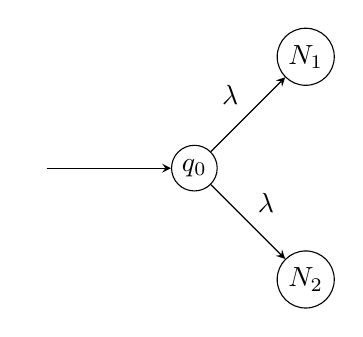
\begin{tikzpicture}[node distance=2cm,on grid,auto]
        \node[state] (0) {\(q_0\)};
        \node (inv) [left=of 0] {};

        \node[state] (a1) [above right=of 0] {\(N_1\)};
        
        \node[state] (b1) [below right=of 0] {\(N_2\)};
        
        \path[->]
            (inv)
                edge node {} (0)
            (0)
                edge node {\(\emptyString\)} (a1)
                edge node {\(\emptyString\)} (b1);
    \end{tikzpicture}
\end{center}

\subsection{Closure under concatenation}

\textit{If \(A\) and \(B\) are two regular languages over the same alphabet
\(\Sigma\), then \(AB\) is also regular.}

Let \(N_1 = (Q_1, \Sigma, \delta_1, q_1, F_1)\) and
\(N_2 = (Q_2, \Sigma, \delta_2, q_2, F_2)\) be two NFAs such that
\(A_1 = L(N_1)\) and \(A_2 = L(N_2)\).
We can construct another NFA \(N=(Q, \Sigma, \delta, q_0, F)\)
such that \(L(N)=AB\).
\(N\) will start by executing \(N_1\), meaning \(q_0=q_1\). If \(N\) switches to a state
\(r\in F_1\) it can move to executing \(N_2\) with a \(\emptyString\)-transition.
The accepted states are only the ones of \(N_2\) meaning \(F=F_2\). \(Q=Q_1 \union Q_2\).
The transition function is hence defined as
\[
    \delta(r, a)
    \begin{cases}
        \delta_1(r, a) & (r \in Q_1 \land r \notin F_1) \lor (r \in F_1 \land r \neq \emptyString) \\
        \delta_1(r, a) \union \{q_2\} & r \in F_1 \land r = \emptyString \\
        \delta_2(r, a) & r \in Q_2
    \end{cases}
\]

\begin{center}
    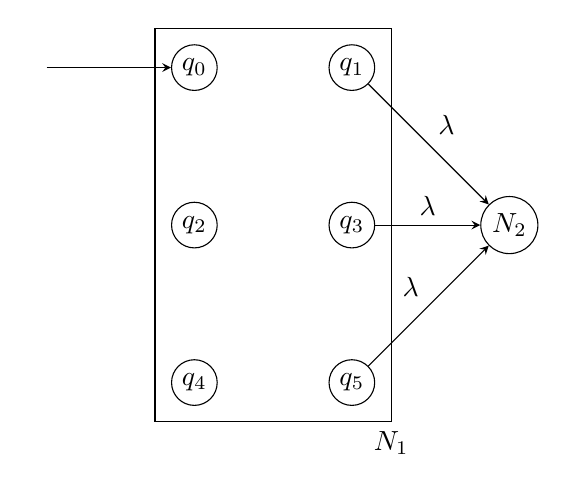
\begin{tikzpicture}[node distance=2cm,on grid,auto]
        \node[state] (q0) {\(q_0\)};
        \node (inv) [left=of q0] {};

        \node[state] (q1) [right=of q0] {\(q_1\)};
        \node[state] (q2) [below=of q0] {\(q_2\)};
        \node[state] (q3) [below=of q1] {\(q_3\)};
        \node[state] (q4) [below=of q2] {\(q_4\)};
        \node[state] (q5) [below=of q3] {\(q_5\)};

        \node[state] (n2) [right=of q3] {\(N_2\)};

        \draw[draw=black] (q0) ++(-0.5, 0.5) rectangle ++(3,-5) node[below] {\(N_1\)};

        \path[->]
            (inv)
                edge node {} (q0)
            (q1)
                edge node {\(\emptyString\)} (n2)
            (q3)
                edge node {\(\emptyString\)} (n2)
            (q5)
                edge node {\(\emptyString\)} (n2);
    \end{tikzpicture}
\end{center}
Here \(F_1 = \{q_1, q_3, q_5\}\) but the actual accept states are the ones for \(N_2\).

\subsection{Closure under Kleene star}

\textit{If \(A\) is a regular language, then \(A^*\) is also regular.}

Let \(N_1 = (Q_1, \Sigma, \delta_1, q_0, F_1)\) be a NFAs such that
\(A_1 = L(N_1)\). We can construct another NFA \(N=(Q, \Sigma, \delta, q, F)\)
such that \(L(N)=A_1^*\).
We want \(N_1\) to be able to switch back to its initial point
when it is in a state \(r \in F_1\). This means that the concatenation of
accepted strings can cycle one after the other. Since \(\emptyString\)
also needs to be accepted we need a new start state which is an accept state.

\begin{itemize}
    \item \(Q = \{q_a\} \union Q_1\)
    \item \(q = q_a\)
    \item \(F = F_1 \union \{q\}\)
    \item \[
        \delta(r,a) =
        \begin{cases}
            \delta_1(r,a) & (r \in Q_1 \land r \notin F_1) \lor (r \in F_1 \land a \neq \emptyString) \\
            \delta_1(r,a) \union \{q_0\} & r \in F_1 \land a = \emptyString \\
            \{q_0\} & r = q \land a = \emptyString \\
            \emptyset & r = q \land a \neq \emptyString
        \end{cases}
    \]
\end{itemize}

\begin{center}
    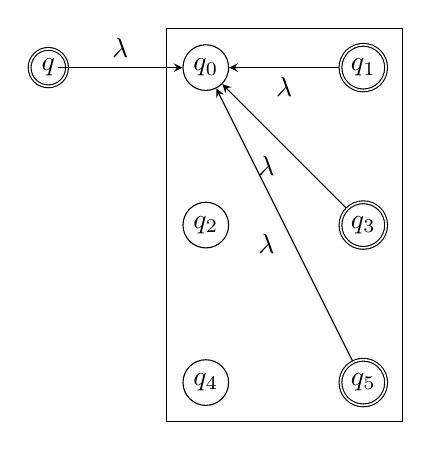
\begin{tikzpicture}[node distance=2cm,on grid,auto]
        \node[state, accepting] (q) {\(q\)};
        \node[state] (q0) [right=of q] {\(q_0\)};
        \node (inv) [left=of q0] {};

        \node[state, accepting] (q1) [right=of q0] {\(q_1\)};
        \node[state] (q2) [below=of q0] {\(q_2\)};
        \node[state, accepting] (q3) [below=of q1] {\(q_3\)};
        \node[state] (q4) [below=of q2] {\(q_4\)};
        \node[state, accepting] (q5) [below=of q3] {\(q_5\)};

        \draw[draw=black] (q0) ++(-0.5, 0.5) rectangle ++(3,-5);

        \path[->]
            (inv)
                edge node {\(\emptyString\)} (q0)
            (q1)
                edge node {\(\emptyString\)} (q0)
            (q3)
                edge node {\(\emptyString\)} (q0)
            (q5)
                edge node {\(\emptyString\)} (q0);
    \end{tikzpicture}
\end{center}

\subsection{Closure under complement}

\textit{If \(A\) is a regular language, then \(\bar{A}\) is also regular.}

Let \(N_1 = (Q_1, \Sigma, \delta_1, q_0, F_1)\) be a NFAs such that
\(A_1 = L(N_1)\). We can construct another NFA \(N=(Q, \Sigma, \delta, q, F)\)
such that \(L(N)=\bar{A_1}\).
Any state \(r \notin F_1\) will be able to switch to a new state \(q_a\),
which is the only accept state of \(N\), with a \(\emptyString\)-transition.
This will negate any accepting state of \(N_1\) and vice versa.

\begin{itemize}
    \item \(Q=\{q_a\} \union Q_1\)
    \item \(q = q_0\)
    \item \(F = \{q_a\}\)
    \item \[
        \delta(r,a) =
        \begin{cases}
            \delta_1(r,a) \union \{q_a\} & r \in F_1 \\
            \delta_1(r,a) & r \notin F_1 \\
        \end{cases}
    \]
\end{itemize}

\begin{center}
    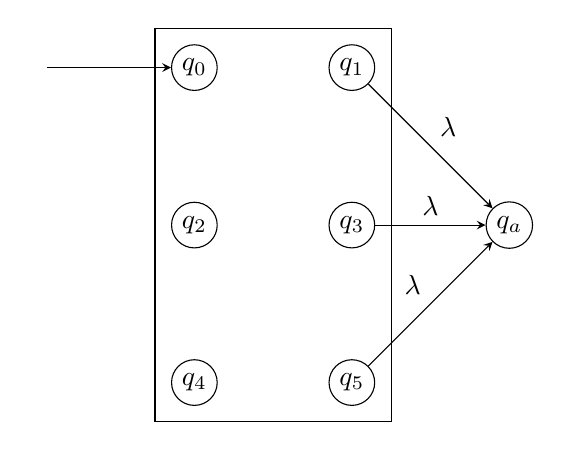
\begin{tikzpicture}[node distance=2cm,on grid,auto]
        \node[state] (q0) {\(q_0\)};
        \node (inv) [left=of q0] {};

        \node[state] (q1) [right=of q0] {\(q_1\)};
        \node[state] (q2) [below=of q0] {\(q_2\)};
        \node[state] (q3) [below=of q1] {\(q_3\)};
        \node[state] (q4) [below=of q2] {\(q_4\)};
        \node[state] (q5) [below=of q3] {\(q_5\)};

        \node[state] (n2) [right=of q3] {\(q_a\)};

        \draw[draw=black] (q0) ++(-0.5, 0.5) rectangle ++(3,-5);

        \path[->]
            (inv)
                edge node {} (q0)
            (q1)
                edge node {\(\emptyString\)} (n2)
            (q3)
                edge node {\(\emptyString\)} (n2)
            (q5)
                edge node {\(\emptyString\)} (n2);
    \end{tikzpicture}
\end{center}
Here \(F_1=\{q_0, q_2, q_4\}\), but the only actual accept state is \(q_a\).

\subsection{Closure under intersection}

\textit{If \(A\) and \(B\) are two regular languages over the same alphabet
\(\Sigma\), then \(A \intersection B\) is also regular.}

Since \(A\union B\) is regular and \(A \intersection B \subseteq A \union B\),
\(A \intersection B\) is also regular.

\section{Regular Expressions}

A regular expression is a mean to express a language.
The class of languages that can be described by
regular expressions coincides with the class of regular languages.

\section{Properties}

Let \(R_1\) be a regular expression describing \(L_1\) and \(R_2\) a regular expression
describing \(L_2\).

\begin{itemize}
    \item \(\emptyString\) is a regular expression describing  \(\{\emptyString\}\)
    \item \(\emptyset\) is a regular expression describing \(\emptyset\)
    \item \(\emptyset^*\) is a regular expression describing \(\{\emptyString\}\)
    \item Let \(\Sigma\) be a non-empty alphabet, \(\forall a \in \Sigma, a\) is a regular expression describing \(\{a\}\)
    \item \(R_1R_2\) is a regular expression describing \(L_1L_2\)
    \item \(R_1\union R_2\) is a regular expression describing \(L_1\union L_2\)
    \item \(R_1\intersection R_2\) is a regular expression describing \(L_1\intersection L_2\)
    \item \(R_1^*\) is a regular expression describing \(L_1^*\)
    \item \(\bar{R_1}\) is a regular expression describing \(\bar{L_1}\)
\end{itemize}
If \(L_1 = L_2\), then we say\(R_1 = R_2\) (e.g. \(\emptyString = \emptyset^*\)).

Let \(R_1, R_2\) and \(R_3\) be regular expressions
\begin{itemize}
    \item \(R_1 \emptyset = \emptyset R_1 = \emptyset\)
    \item \(R_1 \emptyString = \emptyString R_1 = R_1\)
    \item \(R_1 \union R_2 = R_2 \union R_1\)
    \item \(R_1 \union \emptyset = R_1\)
    \item \(R_1 \union R_1 = R_1\)
    \item \(R_1(R_2 \union R_3) = R_1R_2 \union R_1R_3\)
    \item \((R_1 \union R_2)R_3 = R_1R_3 \union R_2R_3\)
    \item \(R_1(R_2R_3) = (R_1R_2)R_3\)
    \item \(\emptyset^*=\emptyString\)
    \item \(\emptyString^*=\emptyString\)
    \item \((\emptyString \union R_1)^* = R_1^*\)
    \item \((\emptyString \union R_1)(\emptyString \union R_1)^* = R_1^*\)
    \item \(R_1^*(\emptyString \union R_1)=(\emptyString \union R_1)R_1^* = R_1^*\)
    \item \(R_1^*R_2 \union R_2 = R_1^*R_2\)
    \item \(R_1(R_2R_1)^*=(R_1R_2)^*R_1\)
    \item \((R_1 \union R_2)^* = (R_1^*R_2)^*R_1^* = (R_2^*R_1)^*R_2^*\)
\end{itemize}

\pagebreak

\section{Equivalence of regular expressions and regular languages}

\subsection{A regular expression describes a regular language}

Let \(R\) be a regular expression over \(\Sigma\).

\begin{wrapfigure}{r}{2.5cm}
    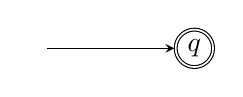
\begin{tikzpicture}[node distance=2cm,on grid,auto]
        \node[state, accepting] (q) {\(q\)};
        \node (inv) [left=of q] {};
    
        \path[->]
            (inv)
                edge node {} (q);
    \end{tikzpicture}
\end{wrapfigure}

Assume that \(R=\emptyString\). Then \(R\) describes \(\{\emptyString\}\).
This language is regular and we can prove it by constructing an NFA \(N=(Q, \Sigma, \delta, q, F)\)
such that \(L(N)=\{\emptyString\}\).
\(q\) is the start state, \(Q=\{q\}\), \(F=\{q\}\) and \(\delta(r,a)=\emptyset\)
where \(a\in\Sigma_\emptyString\).
\wrapfill

\begin{wrapfigure}{r}{2.5cm}
    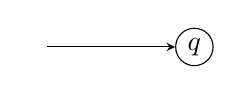
\begin{tikzpicture}[node distance=2cm,on grid,auto]
        \node[state] (q) {\(q\)};
        \node (inv) [left=of q] {};
    
        \path[->]
            (inv)
                edge node {} (q);
    \end{tikzpicture}
\end{wrapfigure}

Assume that \(R=\emptyset\). Then \(R\) describes \(\emptyset\).
This language is regular and we can prove it by constructing an NFA \(N=(Q, \Sigma, \delta, q, F)\)
such that \(L(N)=\emptyset\).
\(q\) is the start state, \(Q=\{q\}\), \(F=\emptyset\) and \(\delta(r,a)=\emptyset\) where \(a\in\Sigma_\emptyString\).
\wrapfill

\begin{wrapfigure}{r}{2.5cm}
    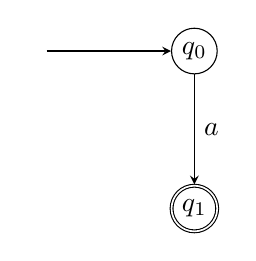
\begin{tikzpicture}[node distance=2cm,on grid,auto]
        \node (inv) {};
        \node[state] (q0) [right=of inv] {\(q_0\)};
        \node[state, accepting] (q1) [below=of q0] {\(q_1\)};
    
        \path[->]
            (inv)
                edge node {} (q0)
            (q0)
                edge node {\(a\)} (q1);
    \end{tikzpicture}
\end{wrapfigure}

Assume that \(R=a\) where \(a\in\Sigma\). Then \(R\) describes \(\{a\}\).
This language is regular and we can prove it by constructing an NFA \(N=(Q, \Sigma, \delta, q, F)\)
such that \(L(N)=\{a\}\).
\(q_0\) is the start state, \(Q=\{q_0, q_1\}\), \(F=\{q_1\}\) and
\[
    \delta(r,b \in) =
    \begin{cases}
        \{q_1\} & b=a \land r=q_0\\
        \emptyset & \text{otherwise}
    \end{cases}
\]
where \(b\in\Sigma_\emptyString\).
\wrapfill

Assume that \(R=R_1 \union R_2\) where \(R_1\) and \(R_2\) are regular expressions.
Let \(L_1\) and \(L_2\) be the languages described by \(R_1\) and \(R_2\) respectively.
Assuming that \(L_1\) and \(L_2\) are regular, \(R\) then describes \(L_1 \union L_2\) which by theorem is regular.

Assume that \(R=R_1 \intersection R_2\) where \(R_1\) and \(R_2\) are regular expressions.
Let \(L_1\) and \(L_2\) be the languages described by \(R_1\) and \(R_2\) respectively.
Assuming that \(L_1\) and \(L_2\) are regular, \(R\) then describes \(L_1 \intersection L_2\) which by theorem is regular.

Assume that \(R=R_1 R_2\) where \(R_1\) and \(R_2\) are regular expressions.
Let \(L_1\) and \(L_2\) be the languages described by \(R_1\) and \(R_2\) respectively.
Assuming that \(L_1\) and \(L_2\) are regular, \(R\) then describes \(L_1 L_2\) which by theorem is regular.

Assume that \(R={(R_1)}^*\) where \(R_1\) is a regular expression. Let \(L_1\) be the language be described
by \(R_1\). Assuming that \(L_1\) is regular, then \(R\) describes \({(L_1)}^*\) which by theorem is regular.

Assume that \(R=\bar{R_1}\) where \(R_1\) is a regular expression. Let \(L_1\) be the language be described
by \(R_1\). Assuming that \(L_1\) is regular, then \(R\) describes \(\bar{L_1}\) which by theorem is regular.

This proves that every regular expression describes a regular language since every
regular expression can be broken down to regular languages.

\subsection{A DFA can be converted into a regular expression}

\subsubsection{Solving recurrence relations}

Let \(\Sigma\) be an alphabet and let \(B\), \(C\) and \(L\) be languages in \(\Sigma^*\) where \(\emptyString \notin B\)
\[
    L=BL\union C \implies L=B^*C
\]

In order to prove this we first show that \(B^*C \subseteq L\) by induction.
Let \(w \in B^*C\), then \(w\) is \(k\geq 0\) strings in \(B\) followed a string in \(C\).
When \(k=0\), \(w \in C\) which implies \(w \in BL\union C\) which implies \(w \in L\).
When \(k > 0\) we can write \(w\) as \(xyz\) where \(x\) is a string in \(B\),
\(y\) is the concatenation of \(k-1\) strings in \(B\) and \(c \in C\).
Let \(q=yz\). Since \(q\) is a concatenation of \(k-1\) strings of \(B\) followed by a string in \(C\),
\(q \in L\). Hence, \(w=xq\) where \(x\in B\) and \(q\in L\). This shows that \(w \in BL\).
Hence, \(w \in BL\union C\). Since \(BL \union C = L\), \(w \in L\). This proves that
\(B^*C\subseteq L\). \\
Now we show that \(L \subseteq B^*C\) by induction to conclude the proof.
Let \(w\in L\). When \(|w|=0\), \(w=\emptyString\). Since \(\emptyString \notin B\),
\(w \notin BL\). This means that \(w\in C\). Since \(C \subseteq B^*C\) the string \(w\)
is also in \(B^*C\). When \(|w| > 0\), if \(w \in C\) then \(w \in B^*C\),
If \(w \notin C\), \(w \in BL\) since \(w \in L\) and \(L=BL\union C\).
Hence, \(w=bl\) where \(b\in B\) and \(l\in L\).
Since \(\emptyString \notin B\), \(|b|>0\). This means that \(|l|<|b|\)
since \(|l|+|b|=|w|\). By induction, \(l\) is a string in \(B^*C\).
Hence, \(w = bl\) where \(b\in B\) and \(l\in B^*C\). This shows that \(w \in B(B^*C)\).
Since \(B(B^*C) \subseteq B^*C\) it follows that \(w \in B^*C\).

\subsubsection{The conversion}

We will now prove that every DFA can be converted into a regular expression.
Let \(M=(Q, \Sigma, \delta, q, F)\) be a DFA. We will prove that there exists a regular
expression describing \(L(M)\).

We define \(L_r\) where \(r \in Q\) as the set of strings \(w \in \Sigma_\emptyString\)
that would be accepted by \(M\) if \(r\) were its start state, meaning the language of \(M\)
if \(r\) were its start state. Note that \(L(M)=L_q\).

\subsection{Conclusion}

Since any DFA \(M\) can be converted into a regular expression that describes \(L(M)\)
and every regular expression describes a regular language, we can conclude that a language \(L\)
is regular iff there exists a regular expression that describes \(L\).

\end{document}

% https://cglab.ca/~michiel/TheoryOfComputation/TheoryOfComputation.pdf
% pag 71